\documentclass[border=7pt]{standalone}
\usepackage{fontspec,unicode-math}
\setmainfont{Noto Serif}
\setmathfont{STIXTwoMath-Regular.otf}
\usepackage{tikz}
\usetikzlibrary{arrows.meta,calc,patterns,decorations.markings,decorations.pathmorphing,decorations.pathreplacing}
\tikzset{lev/.style={line width=1.1pt,line cap=butt},
 fine/.style={line width=.52pt},light/.style={line width=.35pt},
 curve/.style={line width=1.15pt,line cap=round,line join=round},
 ax/.style={line width=.57pt,-{Latex[length=2mm,width=1.15mm]}},
 ray/.style={line width=.58pt,-{Latex[length=1.9mm,width=1mm]},shorten >=1.2pt,shorten <=1.2pt},
 dim/.style={line width=.50pt,{Latex[length=1.65mm,width=.85mm]}-{Latex[length=1.65mm,width=.85mm]}},
 flow/.style={line width=.65pt,postaction={decorate},decoration={markings,mark=at position .6 with {\arrow{Latex[length=1.8mm,width=.95mm]}}}},
 lab/.style={font=\fontsize{12}{14.4}\selectfont,inner sep=1.5pt},
 small/.style={font=\fontsize{10.5}{12.5}\selectfont,inner sep=1.2pt},
 panel/.style={font=\fontsize{12}{14.4}\selectfont\itshape,inner sep=1.5pt}}
\pagestyle{empty}
\begin{document}
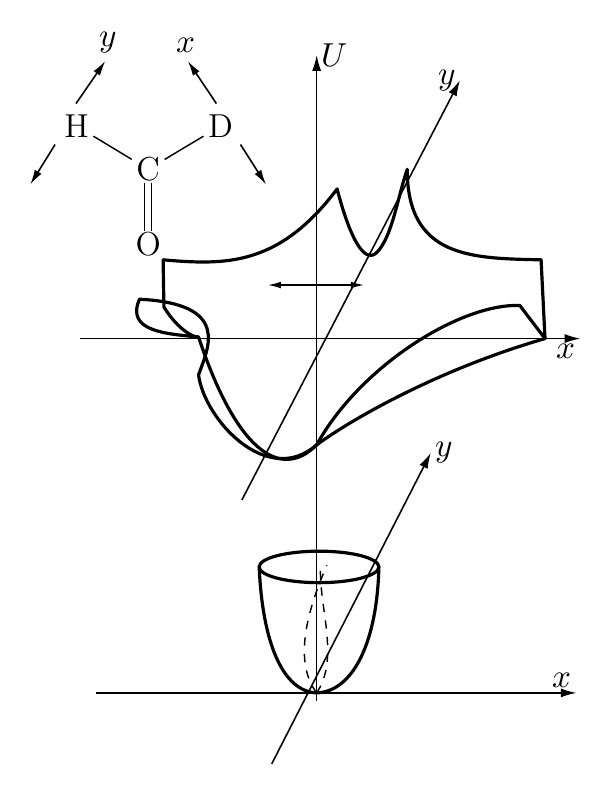
\begin{tikzpicture}[x=1cm,y=1cm,line join=round]

\coordinate (O) at (3.6,0);
\coordinate (E) at (3.6,4.5);
\coordinate (L) at (1.65,5.5);
\coordinate (R) at (6.45,5.5);
\coordinate (C) at (3.6,3.15);
\coordinate (PX) at (6.5,4.5);
\coordinate (PY) at (4.75,6.65);
% Upper electronic term: one continuous outer rim with two distinct ridges,
% respectively feeding the x and y dissociation valleys (schematic geometry).
\draw[curve] (L)
 .. controls (2.45,5.43) and (3.12,5.42) .. (3.86,6.40)
 .. controls (4.01,5.82) and (4.20,5.42) .. (4.37,5.60)
 .. controls (4.56,5.80) and (4.63,6.30) .. (PY)
 .. controls (4.75,5.52) and (5.57,5.52) .. (R);
\draw[curve] (R) -- (PX);
% Two separate lower slopes of upper term. They meet at its same interior valley C.
\draw[curve] (L)--(1.66,4.90)
 .. controls (1.84,4.61) and (2.04,4.51) .. (2.10,4.52)
 .. controls (2.56,3.13) and (3.12,2.67) .. (C)
 .. controls (4.05,3.48) and (5.15,4.11) .. (PX);
% Thin inner contour: author has a distinct bifurcation at the left rim.
\draw[curve] (1.35,5.0)
 .. controls (1.17,4.59) and (1.69,4.56) .. (2.10,4.52);
\draw[curve] (1.35,5.0)
 .. controls (2.52,4.94) and (2.22,4.38) .. (2.10,4.04)
 .. controls (2.17,3.48) and (2.97,2.60) .. (C)
 .. controls (4.15,4.15) and (5.43,4.95) .. (6.18,4.92)
 --(PX);
\draw[ax] (.6,4.5)--(6.95,4.5) node[lab,below left] {$x$};
\draw[ax] (2.65,2.45)--(5.42,7.78) node[lab,left] {$y$};
\draw[ax] (3.6,-.1)--(3.6,8.1) node[lab,right] {$U$};
\draw[fine,densely dashed] (3.6,4.8)--(3.6,5.65);
\draw[dim] (2.98,5.18)--(4.20,5.18);
% Lower electronic term: a bound two-coordinate well.
\draw[curve] (2.87,1.6) .. controls (2.91,.66) and (3.16,.02) .. (O)
 .. controls (4.08,.02) and (4.37,.68) .. (4.39,1.6);
\draw[curve] (3.63,1.6) ellipse (.76 and .20);
\draw[fine,dashed] (O).. controls (3.3,.40) and (3.48,1.05) .. (3.73,1.62);
\draw[fine,dashed] (O).. controls (3.9,.45) and (3.62,1.1) .. (3.65,1.62);
\draw[ax] (.8,0)--(6.9,0) node[lab,above left] {$x$};
\draw[ax] (3.03,-.9)--(5.05,3.05) node[lab,right] {$y$};
% Isotopically asymmetric molecule inset (author's HDCO).
\node[lab] (H) at (.55,7.20) {$\mathrm H$};
\node[lab] (D) at (2.38,7.20) {$\mathrm D$};
\node[lab] (Cmol) at (1.46,6.65) {$\mathrm C$};
\node[lab] (Ox) at (1.46,5.70) {$\mathrm O$};
\draw[fine] (H)--(Cmol)--(D);
\draw[fine] ($(Cmol)+(-.045,-.17)$)--($(Ox)+(-.045,.17)$);
\draw[fine] ($(Cmol)+(.045,-.17)$)--($(Ox)+(.045,.17)$);
\draw[ray] (.52,7.45)--(.94,8.06) node[lab,above] {$y$};
\draw[ray] (.30,7.00)--(-.06,6.42);
\draw[ray] (2.35,7.45)--(1.94,8.06) node[lab,above] {$x$};
\draw[ray] (2.61,7.00)--(2.98,6.42);

\end{tikzpicture}
\end{document}
